%\documentclass[12pt, letterpaper, titlepage]{article}
\documentclass[12pt, letterpaper]{article}

\usepackage{amsmath, amsfonts}
\usepackage{booktabs}
\usepackage{amsthm}
\usepackage{graphicx}
\usepackage[margin=1in]{geometry}
\usepackage{hyperref}
\usepackage{cleveref}
\hypersetup{colorlinks = true, linkcolor = blue, citecolor=blue, urlcolor = blue}
\usepackage{natbib}
\usepackage{float}
\usepackage{setspace}
\usepackage{pdfpages}
\usepackage{lineno}
\usepackage{mwe}
\usepackage{comment}
\linenumbers*[1]
% %% patches to make lineno work better with amsmath
\newcommand*\patchAmsMathEnvironmentForLineno[1]{%
 \expandafter\let\csname old#1\expandafter\endcsname\csname #1\endcsname
 \expandafter\let\csname oldend#1\expandafter\endcsname\csname end#1\endcsname
 \renewenvironment{#1}%
 {\linenomath\csname old#1\endcsname}%
 {\csname oldend#1\endcsname\endlinenomath}}%
\newcommand*\patchBothAmsMathEnvironmentsForLineno[1]{%
 \patchAmsMathEnvironmentForLineno{#1}%
 \patchAmsMathEnvironmentForLineno{#1*}}%

\AtBeginDocument{%
 \patchBothAmsMathEnvironmentsForLineno{equation}%
 \patchBothAmsMathEnvironmentsForLineno{align}%
 \patchBothAmsMathEnvironmentsForLineno{flalign}%
 \patchBothAmsMathEnvironmentsForLineno{alignat}%
 \patchBothAmsMathEnvironmentsForLineno{gather}%
 \patchBothAmsMathEnvironmentsForLineno{multline}%
}

% control floats
\renewcommand\floatpagefraction{.9}
\renewcommand\topfraction{.9}
\renewcommand\bottomfraction{.9}
\renewcommand\textfraction{.1}
\setcounter{totalnumber}{50}
\setcounter{topnumber}{50}
\setcounter{bottomnumber}{50}

\newcommand{\jy}[1]{\textcolor{blue}{JY: #1}}
\newcommand{\eds}[1]{\textcolor{red}{EDS: (#1)}}
\newcommand{\of}[1]{\textcolor{violet}{OF: #1}}

% NOTE: To produce blinded version, replace "0" with "1" below.
\newcommand{\blind}{0}

%\title{On Devon Allen's Disqualification at the 2022 World Track and Field
%Championships}
%
%\author{Owen Fiore\\
%%   \href{mailto:owen.fiore@uconn.edu}
%% {\nolinkurl{owen.fiore@uconn.edu}}\\
  %Elizabeth D. Schifano\\
  %Jun Yan\\[1ex]
  %Department of Statistics, University of Connecticut\\
%}
%\date{}

\begin{document}

\title{\bf Supplement to ``On Devon Allen's Disqualification at the 2022 World Track and Field Championships''}

\if0\blind
{
  \author{Owen Fiore, %\\
%   \href{mailto:owen.fiore@uconn.edu}
% {\nolinkurl{owen.fiore@uconn.edu}}\\
  Elizabeth D. Schifano, %\\
  Jun Yan\\[1ex]
  Department of Statistics, University of Connecticut\\
}
} \fi

\if1\blind
{
  \bigskip
  \bigskip
  \bigskip
  \author{Anonymous Authors}
  \bigskip
} \fi

\maketitle 

\section{Rank-Based Comparison with Pooled Data}

As an alternative to the methods described in Section 3.1 of the main paper, it
is possible to combine all men's and women's reaction time (RT) data for each of 
the three competition
comparisons.  Thus we shrink our analyses from six to three, but each analysis
is roughly twice as big as previously.
For the 2022 national versus
international comparison, there were 160 RTs from 35
athletes and the asymptotic test result was a p-value of $1.94 \cdot 10^{-7}$.
For the 2019 versus 2022 comparison,
there were 258 RTs from 65 athletes and the asymptotic
test result was a p-value of $3.56 \cdot 10^{-8}$. 
For the 2023 versus 2022 comparison, there were 343 RTs
from 92 athletes and the asymptotic test result was a p-value of
$4.99 \cdot 10^{-12}$.  As a result of the larger sample sizes, the code was
very computationally expensive to run and thus we ran it on a smaller size.  All
three permutation tests had a p-value of $1 \cdot 10^{-5}$, which is the smallest
possible value given the permutation test size of $100,000$.  When taken together
with the asymptotic results, the results becoems very clear. These are all
highly significant test results that show substantial differences in average RT
for athletes competing at multiple championship-level events.


\section{GAMLSS Results for Women Data}

We can repeat our reaction time barrier analysis described in Section 3.2, but
fit the same model to women's RT data from 2001 to 2023.
The RT data for women is visualized in Figure~\ref{fig:WomensBoxplot}.
Similar to the men's data, RTs from 2022 appear lower than in other
years. After removing one obvious outliter, which was a disqualfied
reaction time, the same model for men's data fits the women's data
reasonably well.

\begin{figure}[tbp]
  \centering
  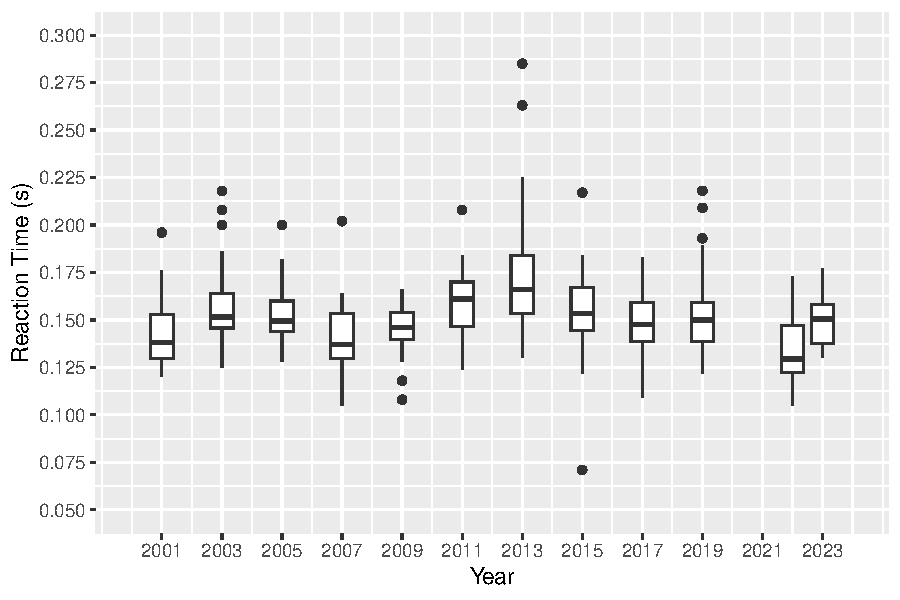
\includegraphics[width=\textwidth]{WomensBoxplot}
  \caption{The RTs from 2021 to 2023 for the women's 100 meter hurdle
  and 100 meter dash.}
  \label{fig:WomensBoxplot}
\end{figure}


\begin{table}
  \centering
  \caption{Estimated fixed-effect parameters with standard errors in
    parentheses and estimated variance of the random effects from the men's and
    women's fitted GG distribution with venue level random
    effects in $\mu$ and heat level random effects in $\sigma$. $n$ denotes
    size of the data.}
  \label{tab:womensfit}
  \begin{tabular}{c c c c c c c}
    \toprule
    Dataset & $n$ & $\beta_0$ & $\gamma_0$ & $\nu$ & $\tau_v$ & $\tau_h$ \\
    \midrule
    Women's & 732 & $-$1.921 (0.007) & $-$2.071 (0.028) & $-$3.691 (0.665) & 0.057 & 0.111 \\
    Men's & 776 & $-$1.910 (0.005) & $-$2.200 (0.027) & $-$1.178 (0.447) & 0.058 & 0.320 \\
    \bottomrule
  \end{tabular}
\end{table}

The fitted parameters in comparison with those from men's data are
summarized in Table~\ref{tab:womensfit}.  One notable aspect is that while
the venue effect standard deviation is nearly identical, the women's heat effect
standard deviation is smaller and $\nu$ is much larger.
This suggests that men’s races exhibit greater 
variability in reaction times, possibly due to faster athletes influencing others 
to react more quickly in certain instances. The consistency in the venue effect 
standard deviation across men’s and women’s data indicates that the venue effect 
is not only statistically significant but also consistent in magnitude across 
genders. These findings highlight the potential impact of competition dynamics 
on heat variability and the robustness of venue-level effects.


\begin{table}
  \centering
  \caption{Probabilities of observing RTs less than threshold 0.08,
  0.09, and 0.10 seconds based on the men's and women's
    fitted GG GAMLSS model with both venue- and heat-level
random effects.}
  \begin{tabular}{c c c c}
   \toprule
   Data Set & Threshold 0.08 & Threshold 0.09 & Threshold 0.10  \\
   \midrule
   Women's & $1\cdot10^{-7}$ & $1.12\cdot10^{-5}$ &  $5.46\cdot10^{-4}$  \\
   Men's   & $6.84\cdot10^{-5}$ & $4.95\cdot10^{-4}$ & $2.76\cdot10^{-3}$ \\
   \bottomrule
  \end{tabular}
  \label{tab:Sim_prob_women}
\end{table}

We can repeat the simulation methods described in the paper to evaluate
the probability of an extreme reaction time.  Table~\ref{tab:Sim_prob_women}
compares the men's and women's results of observing reaction times less than
0.08, 0.09, and 0.1 seconds.  We find that across all three comparisons that
women have a lower probability of having a fast time. The results are slightly
different from those from the men's data, which echoes existing studies
reporting gender differences in RTs \citep[e.g.,][]{lipps2011implications,
babicc2009reaction, panoutsakopoulos2020gender}.



\begin{table}
  \centering
  \caption{Suggested RT barriers based on tail probabilities.}
  \begin{tabular}{c c c c}
   \toprule
   Data Set & Tail probability  $10^{-2}$ & Tail probability  $10^{-3}$ & Tail probability $10^{-4}$ \\
   \midrule
   Women's & $0.111$ & $0.102$ & $0.095$ \\
   Men's   & $0.108$ & $0.094$ & $0.082$ \\
   \bottomrule
  \end{tabular}
  \label{tab:Sim_time_women}
\end{table}

To evaluate a fair reaction time (RT) barrier for women, we compared suggested 
barriers for men and women based on tail probabilities, as shown in 
Table~\ref{tab:Sim_time_women}. The results indicate that men are more likely 
to be disqualified under the current uniform 0.1-second threshold due to their 
generally faster reaction times. This suggests that the same RT standard may not 
have equivalent implications for men and women. Potential adjustments could 
involve raising the barrier for women to align with men’s disqualification rates 
or lowering the barrier for men to match women’s rates. However, further research 
is needed to validate these findings and explore their broader implications. These 
results contribute to ongoing discussions about RT thresholds and emphasize the 
importance of statistical evidence in guiding decisions about competition fairness.


% \section{Results from Data Excluding Positive Disqualified RTs}

% An earlier iteration of the paper fit a model that did not include RTs from
% athletes who were disqualified or did not finish but still registered a RT.  
% However, it was ultimately decided to include these times to better estimate the 
% left tail of the distribution and more accurately predict the probability of a 
% low RT, as described in the main paper.  
% We did not include negative RTs, however, as these represent a mistake 
% of the runner for starting before
% the gun is fired and are thus meaningless in our objective to
% determine a fair RT barrier.  Not all of those disqualified were
% disqualified because of breaking the 0.1 reaction time barrier; there are many
% reasons why an athlete may be disqualified, with the most notable being failed
% drug tests and lane violations.  Nonetheless, in this section,
% we exclude all disqualified RTs to see their effect on the probability of an
% extreme RT.  We fit an identical model to the generalized Gamma model
% presented in Section 3.2 to examine differences results.

% \begin{table}
%   \centering
%   \caption{Probabilities of observing RTs less than threshold 0.08,
%   0.09, and 0.10 seconds based on the
%     fitted GG GAMLSS model with both venue- and heat-level
% random effects.}
%   \begin{tabular}{c c c c}
%    \toprule
%    Data Set & Threshold 0.08 & Threshold 0.09 & Threshold 0.10  \\
%    \midrule
%    Without DQs & $4.93\cdot10^{-5}$ & $3.53\cdot10^{-4}$ &  $1.97\cdot10^{-3}$  \\
%    With DQs & $6.84\cdot10^{-5}$ & $4.95\cdot10^{-4}$ & $2.76\cdot10^{-3}$ \\
%    \bottomrule
%   \end{tabular}
%   \label{tab:DQSim_probability}
% \end{table}

% \jy{Men's data or pooled data?}
% \eds{with or without 2022?}
% \of{I dont know if we have time for this or if this fits the scope of what we
% are working on.}

% Table~\ref{tab:DQSim_probability} shows the effect of removing disqualificated
% times from the analysis.  The probability of observing extreme RTs is lower when
% we remove the 17 observations.

\bibliographystyle{apalike}
\bibliography{citations}


\end{document}
